\section{Lage der Raman-Linien aller Moleküle}
Im Folgenden soll die Lage der Raman-Linien aller gemessenen Moleküle zum besseren Vergleich in 
ein Diagramm \ref{fig:A5} geplottet werden.\\
Zusätzlich wurde in das Diagramm die entsprechenden Literaturwerte geplottet \citep[vgl.][]{zusatzliteratur}. \\
Bei den gemessenen Daten wurde zwischen Polarisation und Depolarisation unterschieden, diese wurde, wie 
im Vorangegangenen Abschnitt bereits erläutert, bestimmt. Die verwendeten Werte sind im Anhang zu finden. Es wurden
allerdings nur die Anti-Stokes Werte verwendet, da diese deutlicher zu erkennen waren und die Zuordnung zu 
den Literaturwerten somit leichter fiel. 
Die Fehler wurden aufgrund der Übersichtlichkeit weggelassen.\\
Wie man an der Grafik \ref{fig:A5} erkennen kann, liegen die gemessenen Linien in der Nähe der theoretischen. 
Jedoch gibt es mehr Linien bei den Literaturwerten, als wie wir gemessen haben. Eine mögliche Erklärung wäre, dass
diese Peaks eine zu geringe Intensität hatten und sie somit nicht als Peak wahrgenommen wurden, sondern wahrscheinlich 
als Hintergrundrauschen interpretiert wurden.
Des Weiteren liegen einige der Literaturwerte 
nahe zusammen, das heißt die Werte die eigentlich zwei (oder drei) verschiedene sind, wurden während dem Versuch als nur ein Wert interpretiert.\\
Zusätzlich ist erkennbar, dass eine Raman-Linie bei jedem Molekül in etwa bei der gleichen
Wellenzahl $\nu \approx 280 \frac{1}{\text{cm}}$ liegt. Somit ist es wahrscheinlich, dass diese 
Raman-Linie mit dem C-Atom in Verbindung steht, da dieses ebenfalls in jedem Molekül vorhanden ist. 
Zudem fällt auf, dass eine weitere Wellenzahl $\nu \approx 650 \frac{1}{\text{cm}}$ öfters in 
Erscheinung tritt, diese ist bei Verbindungen mit einem H-Atom erkennbar. \\
Aber auch die $Cl_3$ Verbindung ist in der Raman-Linie $\nu \approx 780 \frac{1}{\text{cm}}$ 
zu erkennen.\\
Dies soll allerdings im Folgenden noch genauer erläutert werden.
\begin{figure}
    \centering
    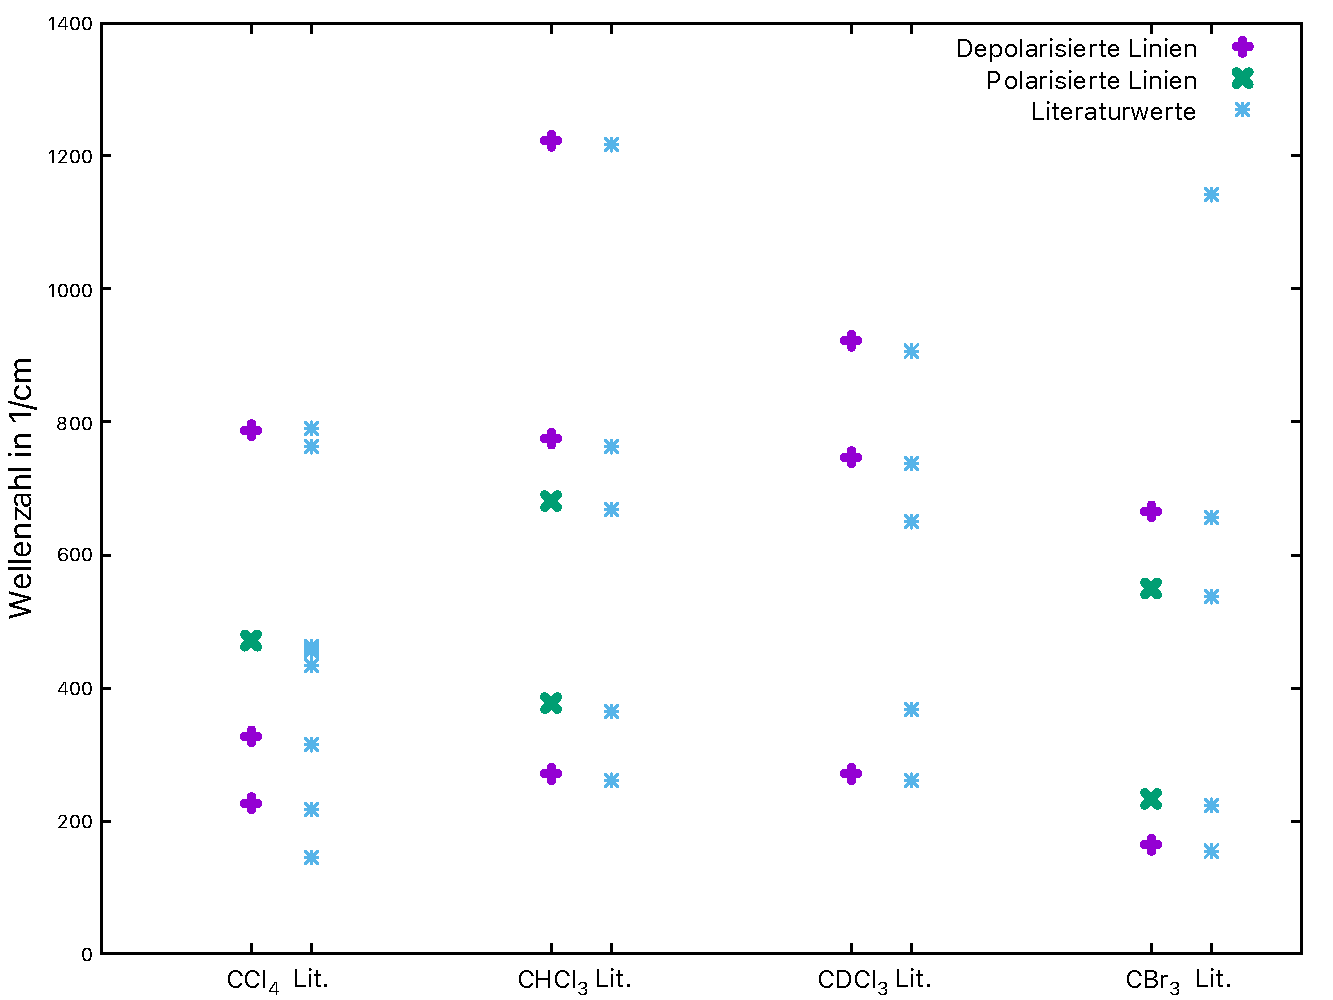
\includegraphics[scale=1, angle=90]{Bilder/Verbesserung_Auswertung/PlotA5.pdf}
    \caption{Lager der Raman Linien für die Moleküle $CHl_3$, $CDCl_3$, $CCl_4$ und $CHBr_3$ mit den entsprechenden Literaturwerten.}
    \label{fig:A5}
\end{figure}
